\chapter{Introduction}\label{intro}

\section{Motivation for Dakota Development}\label{intro:motivation}

Computational models are commonly used in engineering design and
scientific discovery activities for simulating complex physical
systems in disciplines such as fluid mechanics, structural dynamics,
heat transfer, nonlinear structural mechanics, shock physics, and many
others. These simulators can be an enormous aid to engineers who want
to develop an understanding and/or predictive capability for complex
behaviors typically observed in the corresponding physical
systems. Simulators often serve as virtual prototypes, where a set of
predefined system parameters, such as size or location dimensions and
material properties, are adjusted to improve the performance of a
system, as defined by one or more system performance objectives. Such
optimization or tuning of the virtual prototype requires executing the
simulator, evaluating performance objective(s), and adjusting the
system parameters in an iterative, automated, and directed way. System
performance objectives can be formulated, for example, to minimize
weight, cost, or defects; to limit a critical temperature, stress, or
vibration response; or to maximize performance, reliability,
throughput, agility, or design robustness.  In addition, one would
often like to design computer experiments, run parameter studies, or
perform uncertainty quantification (UQ). These approaches reveal how
system performance changes as a design or uncertain input variable
changes.  Sampling strategies are often used in uncertainty
quantification to calculate a distribution on system performance
measures, and to understand which uncertain inputs contribute most to
the variance of the outputs.

A primary goal for Dakota development is to provide engineers and
other disciplinary scientists with a systematic and rapid means to
obtain improved or optimal designs or understand sensitivity or
uncertainty using simulation-based models. These capabilities
generally lead to improved designs and system performance in earlier
design stages, alleviating dependence on physical prototypes and
testing, shortening design cycles, and reducing product development
costs. In addition to providing this practical environment for
answering system performance questions, the Dakota toolkit provides an
extensible platform for the research and rapid prototyping of
customized methods and strategies~\cite{Eld98b}.

\section{Dakota Capabilities}\label{intro:capabilities}

Dakota delivers a variety of iterative methods and strategies, and the
ability to flexibly interface them to your simulation code.  While
Dakota was originally conceived to more readily interface simulation
codes and optimization algorithms, recent versions go beyond
optimization to include other iterative analysis methods such as
uncertainty quantification with nondeterministic propagation methods,
parameter estimation with nonlinear least squares solution methods,
and sensitivity/variance analysis with general-purpose design of
experiments and parameter study capabilities. These capabilities may
be used on their own or as building blocks within more sophisticated
strategies such as hybrid optimization, surrogate-based optimization,
optimization under uncertainty, or mixed aleatory/epistemic UQ.  

The principal classes of Dakota algorithms, with brief descriptions,
are summarized here.  For details, formulations, and usage guidelines,
see the referenced chapters.
\begin{itemize}
\item {\bf Parameter Studies} (Chapter~\ref{ps}): Parameter studies
  employ deterministic designs to explore the effect of parametric
  changes within simulation models.  They can help assess simulation
  characteristics such as smoothness, robustness, and nonlinearity,
  which affect the choice of algorithms and controls in follow-on
  optimization and UQ studies.  Typical examples include centered,
  one-at-a-time variations or joint variation on a grid.

\item {\bf Design of Experiments} (Chapter~\ref{dace}): Design and
  analysis of computer experiments (DACE) techniques are often used to
  explore the parameter space of an engineering design problem, for
  example to perform global sensitivity analysis.  The primary goal of
  these methods is to generate good coverage of the input parameter
  space.  Representative methods include Latin hypercube sampling,
  orthogonal arrays, and Box-Behnken designs.

\item {\bf Uncertainty Quantification} (Chapter~\ref{uq}): Uncertainty
  quantification methods (also referred to as nondeterministic
  analysis methods) compute probabilistic information about response
  functions based on simulations performed according to specified
  input parameter probability distributions.  Put another way, these
  methods perform a forward uncertainty propagation in which
  probability information for input parameters is mapped to
  probability information for output response functions.  Common
  approaches include Monte Carlo sampling, reliability methods, and
  polynomial chaos expansions.

\item {\bf Optimization} (Chapter~\ref{opt}): Optimization solvers
  seek to minimize cost or maximize system performance, as predicted
  by the simulation model, subject to constraints on input variables
  or secondary simulation responses.  Categories of algorithms
  include gradient-based, derivative-free, and global optimization.
  Dakota also includes capabilities for multi-objective trade-off
  optimization and automatic scaling of problem formulations.  Advanced
  Dakota approaches include hybrid (multi-method), multi-start local,
  and Pareto-set optimization.

\item {\bf Calibration} (Chapter~\ref{nls}): Calibration algorithms
  seek to maximize agreement between simulation outputs and
  experimental data (or desired outputs).  They are used solve inverse
  problems (often referred to as parameter estimation or least-squares
  problems).  Dakota approaches include nonlinear least squares and
  Bayesian calibration.

\end{itemize}

Dakota includes a number of related advanced capabilities.  {\bf
  Surrogate models} are inexpensive approximate models that are
intended to capture the salient features of an expensive high-fidelity
model and include data fits, multifidelity, and reduced-order model
surrogates.  They can be used to explore the variations in response
quantities over regions of the parameter space, or they can serve as
inexpensive stand-ins for optimization or uncertainty quantification
studies.  Section~\ref{models:surrogate} summarizes surrogate model
mechanics in Dakota, while optimization methods tailored to particular
surrogate approaches are surveyed in Chapter~\ref{sbm}.

{\bf Nested models} permit layering one Dakota method over another,
enabling algorithms like mixed epistemic-aleatory or second-order UQ,
optimization under uncertainty, or surrogate-based UQ.  Additional
information on these nested approaches is provided in
Section~\ref{models:nested} and Chapter~\ref{adv_models}.

The methods and strategies in Dakota are designed to exploit {\bf
  parallel computing} resources such as those found in a desktop
multiprocessor workstation, a network of workstations, or a massively
parallel computing platform. This parallel computing capability is a
critical technology for rendering real-world engineering design
problems computationally tractable.  See Chapter~\ref{parallel}.

\section{Coupling Dakota to a Simulation}\label{intro:coupling}

A key Dakota advantage is access to a broad range of iterative
capabilities through a single, relatively simple, interface between
Dakota and your simulator. Trying a different iterative method or
strategy typically requires changing only a few commands in the Dakota
text input file, and starting the new analysis.  It does not require
intimate knowledge of the underlying software package integrated in
Dakota, with its unique command syntax and interfacing requirements.
In addition, Dakota will manage concurrent executions of your
computational model in parallel, whether on a desktop or
high-performance cluster computer.

Figure~\ref{intro:bbinterface} depicts a typical loosely-coupled
relationship between Dakota and the simulation code(s).  Such coupling
is often referred to as ``black-box,'' as Dakota has no (or little)
awareness of the internal details of the computational model,
obviating any need for its source code.  Such loose coupling is the
simplest and most common interfacing approach Dakota users
employ. Dakota and the simulation code exchange data by reading and
writing short data files. Dakota is executed with commands that the
user supplies in a text input file (not shown in
Figure~\ref{intro:bbinterface}) which specify the type of analysis to
be performed (e.g., parameter study, optimization, uncertainty
quantification, etc.), along with the file names associated with the
user's simulation code. During operation, Dakota automatically
executes the user's simulation code by creating a separate process
external to Dakota.

\begin{figure}
  \centering
  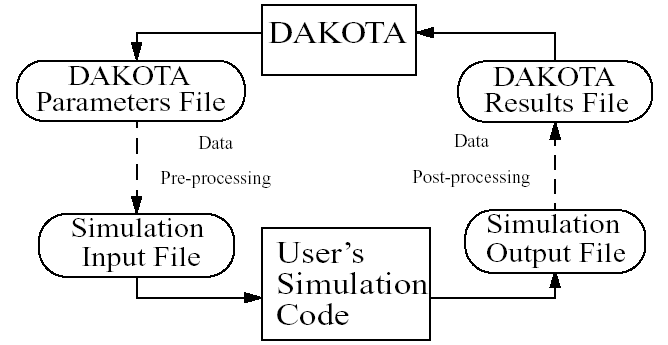
\includegraphics[scale=0.60]{images/dakota_flowchart}
  \caption{The loosely-coupled or ``black-box'' interface between
    Dakota and a user-supplied simulation code.}
  \label{intro:bbinterface}
\end{figure}

The solid lines in Figure~\ref{intro:bbinterface} denote file
input/output (I/O) operations inherent to Dakota or the user's
simulation code. The dotted lines indicate passing or conversion of
information that must be implemented by the user. As Dakota runs, it
writes out a parameters file containing the current variable values.
Dakota then starts the user's simulation code (or, often, a short
driver script wrapping it), and when the simulation completes, reads
the response data from a results file. This process is repeated until
all of the simulation code runs required by the iterative study are
complete.

In some cases it is advantageous to have a close coupling between
Dakota and the simulation code. This close coupling is an advanced
feature of Dakota and is accomplished through either a direct
interface or a SAND (simultaneous analysis and design) interface. For
the direct interface, the user's simulation code is modified to behave
as a function or subroutine under Dakota. This interface can be
considered to be ``semi-intrusive'' in that it requires relatively
minor modifications to the simulation code. Its major advantage is the
elimination of the overhead resulting from file I/O and process
creation. It can also be a useful tool for parallel processing, by
encapsulating all computation in a single executable.  For details on
direct interfacing, see Section~\ref{advint:direct}. A SAND interface
approach is ``fully intrusive'' in that it requires further
modifications to the simulation code so that an optimizer has access
to the internal residual vector and Jacobian matrices computed by the
simulation code. In a SAND approach, both the optimization method and
a nonlinear simulation code are converged simultaneously. While this
approach can greatly reduce the computational expense of optimization,
considerable software development effort must be expended to achieve
this intrusive coupling between SAND optimization methods and the
simulation code.  SAND may be supported in future Dakota releases.


\section{User's Manual Organization}\label{intro:organization}

The Dakota User's Manual is organized into the following major
categories.  New users should consult the Tutorial to get started,
then likely the Method Tour and Interfacing to select a Dakota method
and build an interface to your code.
\begin{itemize}

\item {\bf Tutorial} (Chapter~\ref{tutorial}): How to obtain, install,
  and use Dakota, with a few introductory examples.

\item {\bf Method Tour} (Chapters~\ref{ps} through~\ref{sbm}): Survey
  of the major classes of iterative methods included in Dakota, with
  background, mathematical formulations, usage guidelines, and summary
  of supporting third-party software.

\item {\bf Models} (Chapters~\ref{models} through~\ref{responses}):
  Explanation of Dakota models, which manage the mapping from
  variables through interfaces to responses, as well as details on
  parameter and response file formats for simulation code interfacing.

\item {\bf Input/Output} (Chapters~\ref{input} and~\ref{output}):
  Summary of input to Dakota, including tabular data, and outputs
  generated by Dakota.

\item {\bf Advanced Topics:}
  \begin{itemize}

  \item {\bf Control of Dakota Iteration:} Chapter~\ref{strat}
    addresses strategies and Chapter~\ref{adv_models}, model
    recursions.

  \item {\bf Interfacing:} Chapter~\ref{advint} describes interfacing
    Dakota with engineering simulation codes in both loose- and
    tightly-coupled modes.

  \item {\bf Parallelism:} Chapter~\ref{parallel} described Dakota's
    parallel computing capabilities, with a summary of major
    application parallel modes in Section~\ref{parallel:application}.

  \item {\bf Fault Tolerance:} Chapter~\ref{restart} describes restart
    capabilities and utilities and Chapter~\ref{failure} explains ways
    to detect and mitigate simulation failures.

  \end{itemize}

\item {\bf Additional Examples} (Chapter~\ref{additional}):
  Supplemental example analysis problems and discussion.

\end{itemize}

% LocalWords:  UQ nondeterministic epistemic nonlinearity hypercube Behnken
% LocalWords:  multi multifidelity Jacobian
